%%%%%%%%%%%%%%%%%%%%%%%%%%%%%%%%%%%%%%%%%%%%%%%%%%%%%%%%%%%%%%%%%%
%%%%%%%% ICML 2016 EXAMPLE LATEX SUBMISSION FILE %%%%%%%%%%%%%%%%%
%%%%%%%%%%%%%%%%%%%%%%%%%%%%%%%%%%%%%%%%%%%%%%%%%%%%%%%%%%%%%%%%%%

% Use the following line _only_ if you're still using LaTeX 2.09.
%\documentstyle[icml2016,epsf,natbib]{article}
% If you rely on Latex2e packages, like most moden people use this:
\documentclass{article}

\usepackage{amsmath,amsfonts,amssymb,amsthm,dsfont}
% use Times
\usepackage{times}
% For figures
\usepackage{graphicx} % more modern
%\usepackage{epsfig} % less modern
\usepackage{subfigure} 

% For citations
\usepackage{natbib}

% For algorithms
\usepackage{algorithm}
\usepackage{algorithmic}

% As of 2011, we use the hyperref package to produce hyperlinks in the
% resulting PDF.  If this breaks your system, please commend out the
% following usepackage line and replace \usepackage{icml2016} with
% \usepackage[nohyperref]{icml2016} above.
\usepackage{hyperref}

% Packages hyperref and algorithmic misbehave sometimes.  We can fix
% this with the following command.
\newcommand{\theHalgorithm}{\arabic{algorithm}}

% Employ the following version of the ``usepackage'' statement for
% submitting the draft version of the paper for review.  This will set
% the note in the first column to ``Under review.  Do not distribute.''
\usepackage{icml2016} 

\def\N{\mathbb{N}}
\def\Z{\mathbb{Z}}
\def\R{\mathbb{R}}
\def\C{\mathcal{C}}

\def\e{\varepsilon}
\def\d{\delta}
%\def\w{\omega}
\def\w{\mathrm{w}}
\def\v{\mathrm{V}}
\def\x{\mathrm{x}}
\def\m{\mathrm{m}}
\def\z{\mathrm{z}}

\def\F{\mathcal{F}}
\def\G{\mathcal{G}}
\def\S{\mathcal{S}}
\def\A{\mathcal{A}}
\def\M{\mathcal{M}}

\def\1{\mathds{1}}

\def\KL{\mathrm{KL}}

\def\for{\mbox{  for }}
\def\mle{\mathrm{mle}}
\def\diag{\mathrm{diag}}
\def\cov{\mathrm{cov}}
\def\card{\mathrm{card}}
\def\aff{\mathrm{aff}}
\def\span{\mathrm{span}}
\def\nor{\mathcal{N}}
\DeclareMathOperator*{\argmin}{argmin}

\newtheorem{observation}{Observation}[section]
\newtheorem{theorem}{Theorem}[section]
\newtheorem{proposition}{Proposition}[section]
\newtheorem{lemma}{Lemma}[section]
\newtheorem{corollary}{Corollary}[section]

\theoremstyle{definition}
\newtheorem{definition}{Definition}[section]
\newtheorem{remark}{Remark}[section]
\newtheorem{example}{Example}[section]
\newtheorem{problem}{Problem}[section]


% Employ this version of the ``usepackage'' statement after the paper has
% been accepted, when creating the final version.  This will set the
% note in the first column to ``Proceedings of the...''
%\usepackage[accepted]{icml2016}


% The \icmltitle you define below is probably too long as a header.
% Therefore, a short form for the running title is supplied here:
\icmltitlerunning{Submission and Formatting Instructions for ICML 2016}

\begin{document} 

\twocolumn[
\icmltitle{Submission and Formatting Instructions for \\ 
           International Conference on Machine Learning (ICML 2016)}

% It is OKAY to include author information, even for blind
% submissions: the style file will automatically remove it for you
% unless you've provided the [accepted] option to the icml2016
% package.
\icmlauthor{Your Name}{email@yourdomain.edu}
\icmladdress{Your Fantastic Institute,
            314159 Pi St., Palo Alto, CA 94306 USA}
\icmlauthor{Your CoAuthor's Name}{email@coauthordomain.edu}
\icmladdress{Their Fantastic Institute,
            27182 Exp St., Toronto, ON M6H 2T1 CANADA}

% You may provide any keywords that you 
% find helpful for describing your paper; these are used to populate 
% the "keywords" metadata in the PDF but will not be shown in the document
\icmlkeywords{boring formatting information, machine learning, ICML}

\vskip 0.3in
]

\begin{abstract} 
Independent Component Analysis (ICA) - one of the basic tools in data analysis - aims to find a coordinate system in which the components of the data are independent. In many application the number of sources is unknown and may be less than the number of sensors. In such situation we are looking for so-called non-square mixing matrix.
Due to computational constraints, principal component analysis is used for dimension reduction prior to ICA (PCA+ICA),
which could remove important information.
In this paper we present a two method which are dedicated for determining non-square mixing matrix by fitting non Gaussian densities.
\end{abstract} 



%%%%%%%%%%%%%%%%%%%%%%%%%%%%%%%%
\section{Introduction}
\label{introduction}
%%%%%%%%%%%%%%%%%%%%%%%%%%%%%%%%%%%%%%%%%%%%%%%%%%%%%%%%%%%%%%%%
%%%%%%%%%%%%%%%%%%%%%%%%%%%%%%%%
\section{Introduction}
\label{introduction}
%%%%%%%%%%%%%%%%%%%%%%%%%%%%%%%%

Independent component analysis (ICA) is similar in many aspects to principal component analysis (PCA). In PCA we look for an orthonormal base in which the data components are not
linearly dependent (uncorrelated), while in 
ICA we search for the coordinate system in which the components are independent. More precisely the aim of ICA is to transform the observed data $\X$ into maximally independent components $\S$ with use of an invertible linear transformation $W$, called the {\em transformation matrix}: $$
\S = W^T \X.
$$

Popular ICA methodology does not directly attempt to find components that are independent but rather components that are as non-Gaussian as possible.
This follows from the fact that one of the theoretical foundations of ICA is given by the dual view at the Central Limit Theorem \cite{hyvarinen2000independent}, which states that the distribution of the sum (average or linear combination) of $N$ independent random variables approaches Gaussian as  $N\rightarrow \infty$. Obviously if all source variables are Gaussian, the ICA method will not work. 

Another common approach to ICA based on the maximum likelihood estimation~\cite{pham1997blind} is recently gaining popularity \cite{hyvarinen2004independent,samworth2012independent,ICA2017pattern}.  Then we search for the optimally fitted to data cordinate system $B$ and marginal
densities $f_i$ such that the data density factors in base $B$ as the product of maringal densities. To obtain an efficient method and avoid 
overfitting we have to restrict the marginal densities $f_i$ to a class $\F$ of densities which has not too many parameters which can be easily estimated (clearly from obvious reasons this class has to be different from gaussians).  As $\F$ we typically choose the super-Gaussian logistic density or other heavy tails distributions.

In many applications of ICA we deal with the case when several sensors measure the latents variables and the rest of them record only the noise. This happens when the number of sources is unknown and may be less than the number of sensors (then we are looking for so-called {\em non-square mixing matrix} $W$).
Such a case is common for example in the identification of brain networks
in functional  magnetic resonance imaging (fMRI) 
\cite{beckmann2012modelling,green2002pca}.
%and then we are looking for so-called non-square mixing matrix.
In practice, most approaches deal with this problem by first applying PCA to the observations prior to classic ICA (PCA+ICA) to meet the assumption of square mixing and to reduce computational costs \cite{hyvarinen2004independent}. Although numerically effective, this approach may fail as it is not invariant with respect to linear transformation, since PCA will find a ``noise'' component if
it is sufficiently large. 

%\begin{landscape}
\begin{figure*}[t]
% ensure that we have normalsize text
\normalsize
\begin{center}
\subfigure[Original images 42049 and 220075.] {\label{fig:image_ICA_int_1}
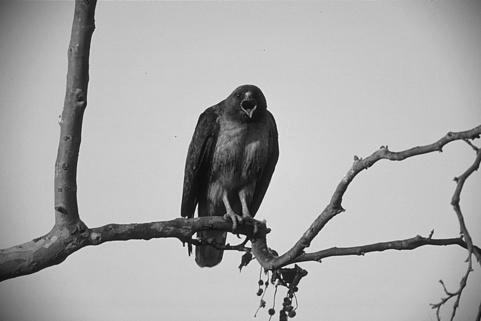
\includegraphics[width=1.6in]{2/2_6_or_1} 
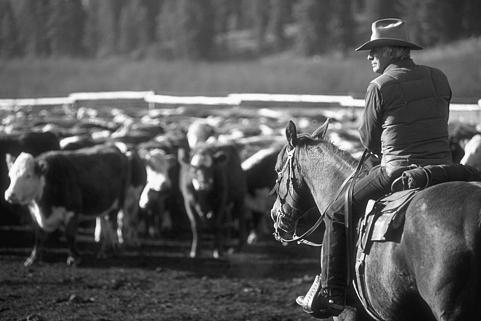
\includegraphics[width=1.6in]{2/2_6_or_2}
}
%%%%%%%%%%%%%%%%%%%%
%\subfigure[Sum and subtraction of images.] {\label{fig:image_ICA_int_2}
%\includegraphics[width=1.2in]{2/2_6_sum} 
%\includegraphics[width=1.2in]{2/2_6_div}
%} \\

%%%%%%%%%%%%%%%%%%%%
\subfigure[\ICA.] {\label{fig:image_ICA_int_3}
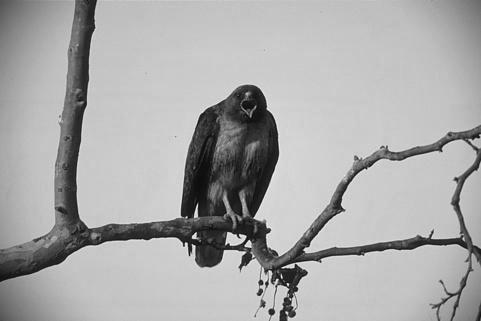
\includegraphics[width=1.6in]{2/2_6_ICA_FEW_II_2} 
}
\subfigure[FastICA.] {\label{fig:image_ICA_int_4}
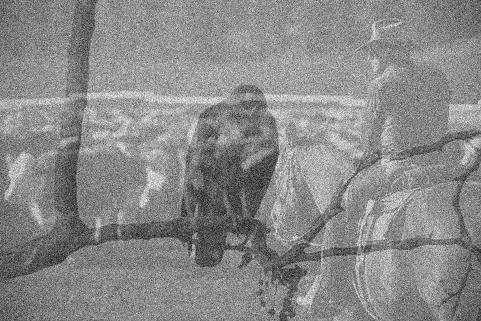
\includegraphics[width=1.6in]{2/2_6_ICA11_2} 
}
\subfigure[ProDenICA.] {\label{fig:image_ICA_int_5}
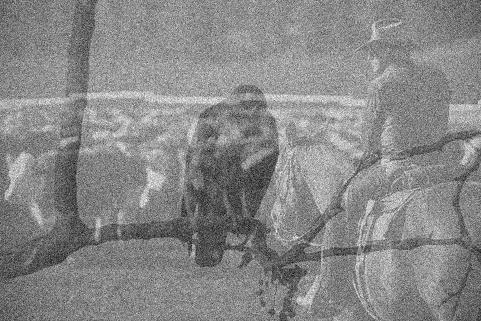
\includegraphics[width=1.6in]{2/2_6_ICA5_2} 
}\\
%%%%%%%%%%%%%%%%%%%%
\subfigure[\ICA.] {\label{fig:image_ICA_int_6}
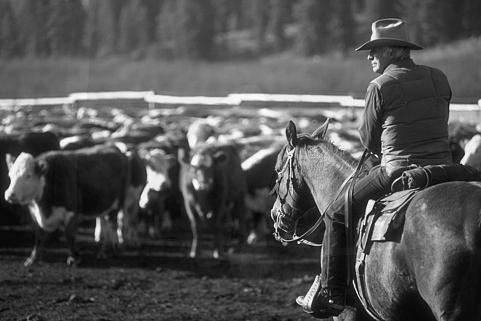
\includegraphics[width=1.6in]{2/2_6_ICA_FEW_II_1}
}
\subfigure[FastICA.] {\label{fig:image_ICA_int_7}
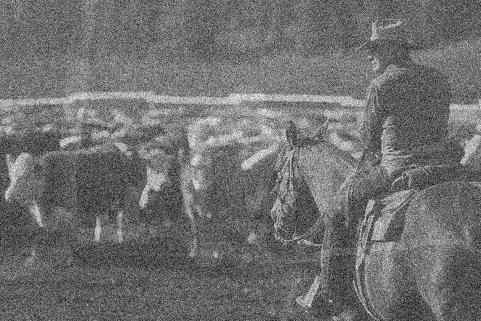
\includegraphics[width=1.6in]{2/2_6_ICA11_1}
}
\subfigure[ProDenICA.] {\label{fig:image_ICA_int_8}
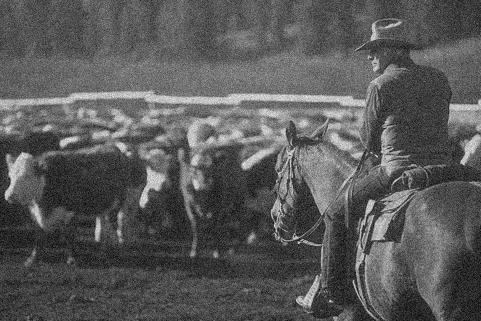
\includegraphics[width=1.6in]{2/2_6_ICA5_1}
}
\end{center}
\caption{Comparison of images separation by our method (\ICA), with FastICA and ProDenICA. Before mixing by a linear matrix, we added to the first two components given in (a) the third component given by random
normal noise. As we see \ICA{} was able to perfectly recover the two first components.}
\label{fig:image_ICA_int}
\end{figure*}

The aim of this paper is to propose a new density based approach to deal with this case which does not have the above
mentioned disadvantage. Our idea is to join the two earlier mentioned approaches to solving ICA - one based on the search for non-gaussian components and the
other based on density estimation - to deal with the case when the number of sources is smaller then that of sensors.  
Observe that the noise typically occurs as a sum of many independent
factors, and consequently thanks to the central limit theorem it typically has approximately gaussian distribution. This is why
one typically makes the assumption \cite{cover2012elements} that
$$
\text{\em noise components are comming from a gaussian noise.}
$$ 
Following the density approach to filter them out we fit the first $d$-components from a class of $\F$ of densities which is broader then gaussians, while the rest from the gaussians $\nor$ (the final choice of the value of parameter $d \in \{1,\ldots,D\}$ can be decided by applying either AIC or BIC criterion). Following \cite{ICA2017pattern} as $\F$ we take the class \SN{} of split-normal densities.

Our experiments show, which is illustrated by Figure \ref{fig:image_ICA_int}, that \ICA{} works as desired and effectively removes the components which contains gaussian noise. However, we cannot objectively conclude that it is better as compared to other state-of-the-art approaches, since the experiment 
was conducted in the setting optimal to our method as we assumed
that the noise was gaussian.

%%%%%%%%%%%%%%%%%%%%%%%%%%%%%%%%
%%%%%%%%%%%%%%%%%%%%%%%%%%%%%%%%
 
%%%%%%%%%%%%%%%%%%%%%%%%%%%%%%%%
\section{basic tools}
\label{sec_1}
%%%%%%%%%%%%%%%%%%%%%%%%%%%%%%%%%%%%%%%%%%%%%%%%%%%%%%%%%%%%%%%%
\subsection{Measure of non-gaussianity}

We are first going to explain the formula \eqref{eq:gen}.
Assume that we have a random vector $\X$ with density $f_\X$. A most common
measure of non-gaussianity is given by the Lullback-Leibler divergence with respect to 
the gaussian measure.
Recall that for a random vector $\X$ finite covariance matrix, its non-Gaussianness is given by
$$
\begin{array}{l}
D(\X)=D(f_\X)=D(f_\X \| \nor(\mean_\X,\cov_\X))\\[1ex]
=\frac{1}{2}\log \det(2\pi e \cov_\X)-h(f_\X),
\end{array}
$$
where $h$ denotes the entropy and $D(f\|g)$ Kullback-Leibler divergence.
It is well-known \cite{cover2012elements} that $D(\X)=0$ iff $\X$ is Gaussian.
Clearly, the above measure is affine invariant.

In practice we have only a finite sample $X$ from $\X$ (that is our data-set). In this case, given a 
family $\F$ of densites on $\R^D$, we can first obtain estimation of the density
by MLE in the class $\F$, and only later compute the measure of nongaussianity. We use the following
notation: given a set $X$, by $\de{X,\F}$ we denote the MLE estimation of the original density $X$ comes from. Thus in this case 
$$
D(X,\F)=\frac{1}{2}\log \det(2\pi e \cov_X)-h(X,\F)
$$ 
is the estimation of the nongaussianity, where $h(X,\F)$ is the estimation of the entropy of $X$
with the use of best estimation from class $\F$: 
$$
h(X,\F)=\frac{1}{\card X}\sum_x -\ln (\de{X,\F}(x)).
$$
Observe that to maximize the above, since the first part is constant, we can minimize
$h(\de{X,\F})$, which is equivalent to maximization of the MLE.

To describe the ability of change of variables, we use the notation based on the push-forward of measures
%
%.Natural method of defining by push-forward
%for more information see \url{https://en.wikipedia.org/wiki/Pushforward_measure},
%\url{http://www.mat.univie.ac.at/~gerald/ftp/book-fa/index.html} (page 256) and
\cite{bogachev2007measure}. Assume that we have a measure on $\R^D$ with density $f$ coming from the random variable $\X$. Then for a linear invertible function $V$, $V\X$ has the density 
$$
V_*f(x)=\frac{1}{|V|} f(V^{-1}y) \text{ for } x \in \R^D.
$$
%Formally it is a push-forward of the measure $\mu$, we denote it by $V_*\mu$, we use
%analogical notation to denote $V_* f$. 
Consider now the case when $f(x_1,\ldots,x_n)=f_1(x_1)\cdot \ldots f_n(x_n)$, that is $f$
is a product measure with respect to base coordinates. In other words, to compute $f(x)$, we can
write
$$
x=x_1 e_1+\ldots +x_n e_n
$$
and compute $f(x)=f_1(x_1) \cdot \ldots \cdot f_n(x_n)$. Now if we want to consider the base given by $V=[\v_1,\ldots,\v_n]$ and the analogue of the above,
we take $x=x_1 \v_1 +\ldots +x_n \v_n$ and 
$$
\frac{1}{\det V} f(x_1) \cdot \ldots \cdot  f(x_n)=V_*f(x).
$$
This is exactly the above.


In our case we will focus our attention on the task of finding $d$ components which are as non-gaussian as possible. For the simplest case, assume that we first consider the first $d$ coordinates, 
and that we want to measure how $X$ is far from being gaussian on the first coordinates. To do so we first need a family $\F_d$ of densities on $\R^d$, which is larger then gaussians. Now we consider
$$
D(X,\F_d \otimes \nor_{D-d}),
$$
where the tensor product of densities is defined by $(f \otimes g)(x,y)=f(x) \cdot g(y)$.

However, in general working with high-dimensional densities, is nontrivial, and therefore for simplicity we fix a family of one dimensional densities that is larger then gaussians $\F$, and take tensor product of $d$-elements of $\F$, that is $\F^{\otimes d}$ (in our case it would be the family of split-gaussians). Thus we search for
$$
\begin{array}{l}
\argmax \limits_V D(X;V_*(\F^{\otimes d} \otimes \nor_{D-d})) \\[1ex]
=\argmin \limits_V h(\de{X,V_*(\F^{\otimes d} \otimes \nor_{D-d}}).
\end{array}
$$
Thus if we reduce to split gaussians of first $d$-dimensions, put $W=V^{-1}$, we get the formulation we described in the introduction.

\medskip

\noindent PROBLEM. {\em Let $X \subset \R^D$ be a data set, and $d \leq D$ be given.
Find a matrix $W=[\w_1,\ldots,\w_D]$, densities $f_1,\ldots,f_d \in \SN$, $f_{d+1},\ldots,f_D \in \nor$, such that 
the likelihood of drawing $X$ from the density
$$
x \to \det(W) \cdot f_1(\w_1^Tx) \cdot \ldots \cdot f_D(\w_D^T x)
$$
is maximized.}

\medskip


%%%%%%%%%%%%%%%%%%%%%%%%%%%%%%%%
%%%%%%%%%%%%%%%%%%%%%%%%%%%%%%%% 
 
%%%%%%%%%%%%%%%%%%%%%%%%%%%%%%%%
\section{przemek}
\label{p}
%%%%%%%%%%%%%%%%%%%%%%%%%%%%%%%%%%%%%%%%%%%%%%%%%%%%%%%%%%%%%%%%


 The density of the one-dimensional Split Gaussian distribution is given by the formula
$$
SN(x;m,\sigma^2,\tau^2) = \left\{ \begin{array}{l}
c \cdot \exp[-\frac{1}{2\sigma^2}(x-m)^2], \textrm{$x\leq m$}\\
c \cdot \exp[-\frac{1}{2\tau^2\sigma^2}(x-m)^2], \textrm{$x>m$}\\
\end{array} \right. \!\!\!\!,
$$
where $c=\sqrt{\frac{2}{\pi}}\sigma^{-1}(1+\tau)^{-1}$. 

A natural generalization of the univariate split normal distribution to the multivariate settings was presented by \cite{villani2006multivariate}.
%\comment{(\cite{john1982three})}
Roughly speaking, authors assume that a vector $\x \in \R^d$ follows the multivariate Split Normal distribution, if its principal components are orthogonal and follow the one-dimensional Split Normal distribution.

\begin{definition}\label{def:SN}
A density of the multivariate Split Normal distribution is given by
$$
 SN_{d}(\x; \m, \sigma,\tau)= \prod_{j=1}^{d} SN(x_j;m_j,\sigma_j^2,\tau_j^2),
$$
where  $\m = [m_1, \ldots, m_d]^T$, $\sigma = [\sigma_{1}^2,\ldots,\sigma_{d}^2]^T$ and $\tau=[\tau_{1}^2,\ldots,\tau_{d}^2]^T$.
%where $W$ is the orthonormal matrix and $\w_{j}$ stand for the $j$-th column of $W$, $\m = (m_1, \ldots, m_d)^T$, $\sigma = (\sigma_{1},\ldots,\sigma_{d})$ and $\tau=(\tau_{1},\ldots,\tau_{d})$.
\end{definition}


In our case we will use density on projection on $d<D$ subspaces. Therefore we need a density $d$-subspace Split Normal distribution.

\begin{definition}\label{def:GSN}
A density of the multivariate $d$-subspace Split Normal distribution is given by
$$
 SN_{d<D}(\x; \m,W, \sigma^2,\tau^2)=  SN_d((W^TW)^{-1}W^T(\x-\m);0,\sigma^2,\tau^2),
$$
where
%%%%%%%%%
$(W^TW)^{-1}W^T(x-m) \in \R^d$
%%%%%%%%%
 $\w_{j} \in \R^D$ is the $j$-th column of non-singular matrix $W = [w_{1},\ldots,w_{d}]$, $\m = [m_1, \ldots, m_D]^T$, $\sigma = [\sigma_{1},\ldots,\sigma_{d}]^T$ and $\tau=[\tau_{1},\ldots,\tau_{d}]^T$.
\end{definition}

Let us recall that the standard Gaussian density in $\R^d$ is defined by 
$$
N(\x;\m,\Sigma)=\frac{1}{(2\pi)^{d/2} \det(\Sigma)^{1/2}} \exp \left(-\tfrac{1}{2} (\x-\m)^T \Sigma^{-1}(\x-\m) \right),
$$
where $\m$ denotes the mean, $\Sigma$ is the covariance matrix.

\begin{definition}\label{def:GSN}
A density of the multivariate $d$-subspace Normal distribution is given by
$$
 N_{d<D}(\x; \m, \Sigma, W)= N((W^TW)^{-1}W^T(\x-\m);0,\Sigma),
$$
where
%%%%%%%%%
$(W^TW)^{-1}W^T(\x-\m) \in \R^d$
%%%%%%%%%
 $\w_{j} \in \R^D$ is the $j$-th column of non-singular matrix $W = [w_{1},\ldots,w_{d}]$, $\m = [m_1, \ldots, m_D]^T$, $\Sigma = \diag(\sigma_{1}^2,\ldots,\sigma_{d}^2)$.
\end{definition}

Our goal is to minimize
$$
\KL(X,\F,\G)=\mle(X,\F)-\mle(X,\G) 
$$
In our language
\begin{equation}
\begin{array}{l}
\KL_{d<D}(X;\m,W,\sigma,\tau,\Sigma) = \\[6pt]
= \sum \limits_{\x \in X} \ln(SN_{d<D}(\x;\m,W,\sigma,\tau)) -
   \sum \limits_{\x \in X} \ln(N_{d<D}(\x;\m,\Sigma,W))
\end{array}
\end{equation}
We known
$$
\sum \limits_{\x \in X} \ln(N_{d<D}(\x;\m,\Sigma,W)) = -\frac{d}{2}\ln(2\pi e)-\frac{1}{2}\ln \det(\Sigma_{W}), 
$$
where 
$$
\Sigma_{W} = \cov( \{ (W^TW)^{-1}W^T(\x-\m) \colon \x \in \R^D\} )
$$

%%%%%%%%%%%%%%%%%%%
\subsection{Optimization problem}
%%%%%%%%%%%%%%%%%%%

The density of the multivariate d-subspace Normal distribution depends on four parameters $\m \in \R^d$, $W \in \M(\R^d)$, $\sigma \in \R^d$, $\tau \in \R^d$. 
We can find them by minimizing the simpler function, which depends on only  $m \in \R^d$ and $W \in \M(\R^d)$. Other parameters are given by explicit formulas. Let us notice that in this case our minimization problem simplifies to minimizing the function $\mle(X,\F) = \sum \limits_{\x \in X} \ln(SN_{d<D}(\x;\m,W,\sigma,\tau))$

\begin{theorem}\label{the:min}
Let $\x_1,\ldots,\x_n$ be given.  
Then the likelihood maximized w.r.t. $\sigma$ and $\tau$ is
\begin{equation}\label{eq:1}
%\min_{\sigma, \tau}
 \hat{L}(X;\m,W) =   \bigg( \frac{2n}{\pi e} \bigg)^{dn/2} \bigg( \prod_{j=1}^{d} g_{j}(\m,W) \bigg)^{-3n/2},
\end{equation}
where
$$
\begin{array}{c}
{g}_{j}(\m,W) = {s}_{1j}^{1/3} + {s}_{2j}^{1/3},
%\\[1ex]
%W_{\omega}=(W^TW)^{-1}W^T,
\\[1ex]
{s}_{1j}= \! \sum\limits_{i \in I_j}[ \w_{j}^T (\x_i-\m)]^2,  {I}_j=\{ i = 1,\ldots,n \colon \w_{j}^T (\x_i-\m) \leq 0 \},
\\[1ex]
{s}_{2j}= \! \sum\limits_{i \in I_j^c}[ \w_{j}^T (\x_i-\m)]^2, {I}_j^c=\{ i = 1,\ldots,n \colon  \w_{j}^T (\x_i-\m) > 0 \},
\end{array}
$$
where $\omega_j$ is the $j$-th column of non-singular matrix $(W^TW)^{-1}W^T$ and the maximum likelihood estimators of $\sigma_{j}^2$ and $\tau_{j}$ are
$$\hat \sigma_j^2(\m,W) = \tfrac{1}{n} s_{1j}^{2/3} g_{j}(\m,W), \quad
\hat \tau_{j}(\m,W)=\left(\frac{s_{2j}}{s_{1j}}\right)^{1/3}.
$$
\end{theorem}

\begin{proof}[Proof of Theorem \ref{the:min}.]
Let $X=\{ \x_1, \ldots, \x_n \}$ and $W_{\omega}=(W^TW)^{-1}W^T$.
We write 
$$
\z_i=  W_{\omega}(\x_i-m), \quad \z_{ij}= \omega_j^T(\x_i-m),
$$
for observation $i$, where $i=1,\ldots,n$ and coordinates $j=1,\ldots,d$.

Let us consider the likelihood function, i.e. 
$$
\begin{array}{l}
L(X;\m,W,\sigma,\tau) = \prod\limits_{i=1}^n SN_{d<D}(\x_i;\m,W,\sigma,\tau) =  
%= \sum \limits_{\x \in X} \ln(SN_{d<D}(\x;\m,W,\sigma,\tau)) 
\prod\limits_{i=1}^{n} \prod\limits_{j=1}^{d} SN(\omega_j^T(\x_i - \m) ; 0,\sigma^2,\tau^2)
\\[6pt]
= c_1^n \Big( \prod\limits_{j=1}^{d} \sigma_j(1+\tau_j) \Big)^{-n} %\cdot \\[6pt]
\prod\limits_{i=1}^{n} \prod\limits_{j=1}^{d} \exp \Big[ -\frac{1}{2\sigma_j^2}z_{ij}^2 (\1_{ \{ z_{ij} \leq 0 \} } + \tau_{j}^{-2} \1_{ \{ z_{ij} > 0 \} }) \Big],
\end{array}
$$
%$$
%\begin{array}{l}
%= \prod\limits_{i=1}^{n} GSN_d(\x_i ; \m,V,\sigma,\tau)
%= \prod\limits_{i=1}^{n} \frac{1}{| \det( V)|}  \prod\limits_{j=1}^{d} SN(  \v^{-1}_j \x_i ; \v^{-1}_j \m , \sigma_j^2, \tau_j^2)=
%\\[1ex]
%\left(\frac{c_1}{|\det(V)|}\right)^{n} \left( \prod\limits_{j=1}^{d} \sigma_j(1+\tau_j) \right)^{-n} \left( \prod\limits_{i=1}^{n} \prod\limits_{j=1}^{d} \exp[-\frac{1}{2\sigma_j^2}z_{ij}^2 (\1_{ \{ z_{ij} \leq 0 \} } + \tau_{j}^{-2} \1_{ \{ z_{ij} > 0 \} })]\right)
%\end{array}
%$$
where 
$
c_1=\left( \sqrt{\tfrac{2}{\pi}} \right)^{d}.
$
Now we take the log-likelihood function, i.e.
$$
\begin{array}{l}
\ln(L(X;\m,W,\sigma,\tau)) \\[6pt]
=\ln \bigg( c_1^n \Big( \prod\limits_{j=1}^{d} \sigma_j(1+\tau_j) \Big)^{-n} \bigg) + %\\[6pt]
 \sum\limits_{i=1}^{n} \sum\limits_{j=1}^{d} \Big[ -\frac{1}{2\sigma_j^2}z_{ij}^2 (\1_{ \{ z_{ij} \leq 0 \} } + \tau_{j}^{-2} \1_{ \{ z_{ij} > 0 \} })\Big]  \\[6pt]
= \ln \bigg( c_1^n \Big( \prod\limits_{j=1}^{d} \sigma_j(1+\tau_j) \Big)^{-n} \bigg)  -%\\[6pt]
  \frac{1}{2} \sum\limits_{j=1}^{d} \Big( \sigma_j^{-2} \sum\limits_{i \in I_{j}}    z_{ij}^2   + \frac{\sigma_j^{-2}}{\tau_{j}^{2} }  \sum\limits_{i \in I_{j}^{c}}   z_{ij}^2  \Big) \\[6pt]
= \ln \bigg( c_1^n \Big( \prod\limits_{j=1}^{d} \sigma_j(1+\tau_j) \Big)^{-n} \bigg)  - 
 \sum\limits_{j=1}^{d} \frac{1}{2\sigma_j^{2}} \Big(  s_{1j}  + \frac{1}{\tau_{j}^{2} }  s_{2j}  \Big).
\end{array}
$$

We fix  $\m$, $W$ and maximize the log-likelihood function over $\tau$ and $\sigma$.
In such a case we have to solve the following system of equations
$$
\begin{array}{l}
\frac{\partial  \ln ( L(X;\m,W,\sigma,\tau) ) }{\partial \sigma_j} = -\frac{n}{\sigma_j} +  \sigma_j^{-3} (s_{1j} + \tau_j^{-2} s_{2j} )
 =0, \\[6pt] %& \mbox{ for }  & j=1,\ldots,d,
 \frac{\partial  \ln ( L(X;\m,W,\sigma,\tau) ) }{\partial \tau_j} = - \frac{n}{1+\tau_j} + \frac{s_{2j}}{\tau_j^{3}\sigma_j^{2}} =0 , %& \mbox{ for }  & j=1,\ldots,d.
\end{array}
$$
for  $ j=1,\ldots,d$.
By simple calculations we obtain the expressions for the estimators
%\begin{align*}
$$
\hat{\sigma}_j^2(\m,W) = 
\tfrac{1}{n} s_{1j}^{2/3} g_{j}(\m,W), \qquad
\hat{\tau}_{j}(\m,W) = \bigg( \frac{s_{2j}}{s_{1j}} \bigg)^{1/3}.
$$
%\end{align*}
Substituting it into the log-likelihood function,
%and taking $e^{\ln \hat{L}(\m,W)}$
we get
$$
\begin{array}{l}
\hat{L}(\m,W) = \bigg( \frac{2}{\pi} \bigg)^{\frac{dn}{2}} \Big( \prod\limits_{j=1}^{d} \frac{1}{\sqrt{n}} g_j(\m,W)^{\frac{3}{2}} \Big)^{-n}  e^{-\frac{dn}{2}}\\[6pt]
= \bigg( \frac{2n}{\pi e} \bigg)^{\frac{dn}{2}}  \Big( \prod\limits_{j=1}^{d} g_j(\m,W) \Big)^{-\frac{3n}{2}}. 
\end{array}
$$
\end{proof}

%\begin{theorem}\label{the:Villani}
%Given a random sample $\x_1,\ldots,\x_n$ from $SN(\mu,\lambda^2,\tau^2)$, the likelihood, maximized over $\lambda$ and $\tau$, is
%\begin{equation}\label{eq:Villani}
%%\min_{\sigma, \tau}
% \hat{L}(\mu) =   \bigg( \frac{2n}{\pi e} \bigg)^{n/2} \bigg( \prod_{j=1}^{d} g_{j}(\m,W) \bigg)^{-3n/2},
%\end{equation}
%where
%$$
%\begin{array}{c}
%{g}_{j}(\m,W) = {s}_{1j}^{1/3} + {s}_{2j}^{1/3},
%\\[1ex]
%{s}_{1j}= \! \sum\limits_{i \in I_j}[ \w_{j}^T (\x_i-\m)]^2,  {I}_j=\{ i = 1,\ldots,n \colon \w_{j}^T (\x_i-\m) \leq 0 \},
%\\[1ex]
%{s}_{2j}= \! \sum\limits_{i \in I_j^c}[ \w_{j}^T (\x_i-\m)]^2, {I}_j^c=\{ i = 1,\ldots,n \colon  \w_{j}^T (\x_i-\m) > 0 \},
%\end{array}
%$$
%and the maximum likelihood estimators of $\sigma_{j}^2$ and $\tau_{j}$ are
%$$\hat \sigma_j^2(\m,W) = \tfrac{1}{n} s_{1j}^{2/3} g_{j}(\m,W), \quad
%\hat \tau_{j}(\m,W)=\left(\frac{s_{2j}}{s_{1j}}\right)^{1/3}.
%$$
%\end{theorem}


Thanks to the above theorem, instead of looking for the maximum of the likelihood function, it is enough to obtain the maximum of the simpler function~(\ref{eq:1}) which depends on two parameters $\m \in \R^d$ and $W \in \M(\R^d)$
\begin{equation}\label{equ:ll}
{l}(X;\m,W) = \prod_{j=1}^{d} {g}_{j}(\m,W)
\end{equation}
where $\w_{j}$ stands for the $j$-th column of matrix $W$. 
Consequently, maximization of (\ref{eq:1}) is equivalent to minimization of  (\ref{equ:ll}), see the following corollary.

\begin{corollary}\label{c2}
Let $X \subset \R^d$, $\m \in \R^d$, $W \in \M(\R^d)$ be given, then
$$
 \text{argmax}_{\m,W} \hat{L}(X;\m,W) =  \argmin_{\m,W} {l}(X;\m,W).
$$
\end{corollary}
%\begin{proof}
%Notice that $l(\m,V,X) = l(\m,W^{-1},X)= {l}(X;\m,W)$ where $W=V^{-1}$ and $$
%\argmax_{\m,V} \hat L(\m,V,X) = \argmin_{\m,V} l(\m,V,X).
%$$
%Moreover
%$$
%\min_{\m,V} l(\m,V,X) = \min_{\m,W} {l}(X;\m,W).
%$$
%
%\end{proof} 


%%%%%%%%%%%%%%%%%%%
\subsection{Gradient}
%%%%%%%%%%%%%%%%%%%

%Minimization of 

%In this subsection we calculate the gradient of the function $\ln({l})$.

One of the possible methods of optimization is the gradient method. Since the minimum of ${l}$ is equal to the minimum of $\ln({l})$, in this subsection we calculate the gradient of $\ln({l})$. 
Before we prove suitable Theorem \ref{ther:grad}, we recall the following lemma. 

\begin{lemma}\label{jacobi}
%\comment{Jacek mowi, ze powino być A(t), i napisać co to znaczy adj()}
Let $A = (a_{ij})_{1 \leq i,j \leq d}$ be a differentiable map from real numbers to $d \times d$ matrices then
\begin{equation}
\frac{\partial \det(A)}{\partial a_{ij}} = \mathrm{adj}^T(A)_{ij},
\end{equation}
where $\mathrm{adj}(A)$ stands for the adjugate of $A$, i.e. the transpose of the cofactor matrix.
\end{lemma}
\begin{proof}
By the Laplace expansion $\det A = \sum\limits_{j=1}^{d} (-1)^{i+j} a_{ij} M_{ij}$ where $M_{ij}$ is the minor of the entry in the $i$-th row and $j$-th column. Hence
$$\frac{\partial \det A}{\partial a_{ij}} = (-1)^{i+j} M_{ij} = \mathrm{adj}^T(A)_{ij}.$$
\end{proof}
Now we are ready to calculate gradient of our cost function.

\begin{theorem}\label{ther:grad}
Let $X \subset \R^d$, $\m = (\m_1, \ldots, \m_d)^T \in \R^d$, $W = (\w_{ij})_{1 \leq i,j \leq d}$ non-singular be given. 
Then
$\nabla_{\m}  \ln {l}(X;\m,W) = \left(  \frac{\partial \ln {l}(X;\m,W)}{\partial \m_1}, \ldots, \frac{\partial \ln {l}(X;\m,W)}{\partial \m_d} \right)^T$,
where
$$
\begin{array}{l}
\frac{\partial \ln {l}(X;\m,W)}{\partial \m_k} =
\sum \limits_{j=1}^d \frac{-1}{{s}_{1j}^{\frac{1}{3}} + {s}_{2j}^{\frac{1}{3}}} \bigg(
\frac{1}{3 {s}_{1j}^{\frac{2}{3}}} \sum \limits_{i \in I_j} 2 \w_j^T (\x_i - \m)  \w_{jk} + %\\[6pt]
\frac{1}{3 {s}_{2j}^{\frac{2}{3}}} \sum \limits_{i \in I_j^c} 2 \w_j^T (\x_i - \m)  \w_{jk}
\bigg).
\end{array}
$$
Moreover,
$
\nabla_{W} \ln {l}(X;\m,W) = \left[ \frac{\partial \ln \tilde{l}(X;\m,W)}{\partial \w_{pk}}  \right]_{1 \leq p,k \leq d},
$
where
$$
\begin{array}{l}
\frac{\partial \ln \tilde{l}(X;\m,W)}{\partial \w_{pk}}  = 
-\frac{2}{3}  (\w^{-1})^T_{pk} +%\\[6pt] 
\frac{1}{{s}_{1p}^{\frac{1}{3}} +{s}_{2p}^{\frac{1}{3}}} 
\bigg(
\frac{1}{3} {s}_{1p}^{-\frac{2}{3}}  \sum \limits_{i \in {I}_p} 2 \w^T_p  (\x_i - \m) (\x_{ik} - \m_k) + \\[6pt]
+ \frac{1}{3} {s}_{2p}^{-\frac{2}{3}}  \sum \limits_{i \in {I}_p^c} 2 \w^T_p  (\x_i - \m) (\x_{ik} - \m_k) \bigg).
\end{array}
$$
and
$$
\begin{array}{c}
%{g}_{j}(\m,W) = {s}_{1j}^{1/3} + {s}_{2j}^{1/3},
%\\[1ex]
{s}_{1j}= \! \sum\limits_{i \in I_j}[ \w_{j}^T (\x_i-\m)]^2, {I}_j=\{ i = 1,\ldots,n \colon \w_{j}^T (\x_i-\m) \leq 0 \},
\\[1ex]
{s}_{2j}= \! \sum\limits_{i \in I_j^c}[ \w_{j}^T (\x_i-\m)]^2,  {I}_j^c=\{ i = 1,\ldots,n \colon  \w_{j}^T (\x_i-\m) > 0 \}.
\end{array}
$$
\end{theorem}

\begin{proof}[Proof of Theorem \ref{ther:grad}.]
Let us start with the partial derivative of $\ln({l})$ with respect to $\m$. We have
$$
\begin{array}{l}
\frac{\partial \ln {l}(X;\m,W)}{\partial \m_k} =
\sum \limits_{j=1}^d \frac{\partial \ln ({g}_j(\m,W))}{\partial \m_k} = \sum\limits_{j=1}^d \frac{1}{{s}_{1j}^{\frac{1}{3}} + {s}_{2j}^{\frac{1}{3}}} \frac{\partial ({s}_{1j}^{\frac{1}{3}} + {s}_{2j}^{\frac{1}{3}})}{\partial \m_k} %=\\[6pt]
 \sum \limits_{j=1}^d \frac{1}{{s}_{1j}^{\frac{1}{3}} + {s}_{2j}^{\frac{1}{3}}} \bigg(
\frac{1}{3 {s}_{1j}^{\frac{2}{3}}} \frac{\partial {s}_{1j}}{\partial \m_k} +
\frac{1}{3 {s}_{2j}^{\frac{2}{3}}} \frac{\partial {s}_{2j}}{\partial \m_k}
\bigg).
\end{array}
$$
Now, we need $\frac{\partial {s}_{1j}}{\partial \m_k}$ and $\frac{\partial {s}_{2j}}{\partial \m_k}$, therefore
$$
\begin{array}{l}
\frac{\partial {s}_{1j}}{\partial \m_k} = 
\sum\limits_{i \in {I}_j} \frac{\partial [\w^T_j (\x_i - \m)]^2}{\partial \m_k} = \sum\limits_{i \in {I}_j} 2 \w^T_j (\x_i - \m) \frac{\partial \w^T_j (\x_i - \m)}{\partial \m_k} = %\\[6pt]
 \sum\limits_{i \in {I}_j} - 2 \w^T_j (\x_i - \m) \w_{jk}.
\end{array}
$$
Analogously we get
$$
\begin{array}{l}
\frac{\partial {s}_{2j}}{\partial \m_k} = \sum\limits_{i \in {I}_j^c} -2 \w^T_j (\x_i - \m) \w_{jk}.
\end{array}
$$
%\comment{$\v^{-1}_{jk} = \w_{jk}$}\\
Hence 
$$
\begin{array}{l}
\frac{\partial \ln {l}}{\partial \m_k} =\sum\limits_{j=1}^d \frac{-1}{{s}_{1j}^{\frac{1}{3}} + {s}_{2j}^{\frac{1}{3}}} \bigg(
\frac{1}{3 {s}_{1j}^{\frac{2}{3}}} \sum\limits_{i \in I_j} 2 \w_j^T (\x_i - \m)  \w_{jk} +% \\[6pt]
\frac{1}{3 {s}_{2j}^{\frac{2}{3}}} \sum\limits_{i \in I_j^c} 2 \w_j^T (\x_i - \m) \w_{jk}
\bigg).
\end{array}
$$

Now we calculate the partial derivative of $\ln {l}(X;\m,W)$ with respect to the matrix $W$. We have
$$
\begin{array}{l}
\frac{\partial \ln {l}(X;\m,W)}{\partial \w_{pk}} = \frac{\partial \ln |\det(W)|^{-\frac{2}{3}}}{\partial \w_{pk}} + \sum\limits_{j=1}^d \frac{\partial \ln ({g}_j(\m,W))}{\partial \w_{pk}}.
\end{array}
$$
%\comment{$\v_{pk}^{-1} = \w_{pk}$}\\
To calculate the derivative of the determinant we use Jacobi's formula (see Lemma \ref{jacobi}).
Hence% $\frac{\partial \ln (\det(W)^{-\frac{2}{3}})}{\partial \w_{pk}} =$
$$
\begin{array}{l}
\frac{\partial \ln (\det(W)^{-\frac{2}{3}})}{\partial \w_{pk}} = \det(W)^{\frac{2}{3}}  \Big(-\frac{2}{3}\Big)  \det(W)^{-\frac{5}{3}}  \frac{\partial \det(W)}{\partial \w_{pk}} = -\frac{2}{3} \det(W)^{-1}  \mathrm{adj}^T(W)_{pk} \\[6pt]
 = -\frac{2}{3} \frac{1}{\det(W)}  \left[\det(W)  (W^{-1})^T_{pk}\right]= -\frac{2}{3}  (\w^{-1})^T_{pk},
\end{array}
$$
where $(\w^{-1})^T_{pk}$ is the element in the $p$-th row and $k$-th column of the matrix $(W^{-1})^T$. Now we calculate %$\frac{\partial \ln ({g}_j(\m,W))}{\partial \w_{pk}} =$
$$
\begin{array}{l}
\frac{\partial \ln ({g}_j(\m,W))}{\partial \w_{pk}} = \frac{1}{{s}_{1j}^{\frac{1}{3}} + {s}_{2j}^{\frac{1}{3}}} \frac{\partial ({s}_{1j}^{\frac{1}{3}} + {s}_{2j}^{\frac{1}{3}})}{\partial \w_{pk}}= \frac{1}{{s}_{1j}^{\frac{1}{3}} + {s}_{2j}^{\frac{1}{3}}} \bigg(
\frac{1}{3 {s}_{1j}^{\frac{2}{3}}}  \frac{\partial {s}_{1j}}{\partial \w_{pk}} +
\frac{1}{3 {s}_{2j}^{\frac{2}{3}}}  \frac{\partial {s}_{2j}}{\partial \w_{pk}}
\bigg),
\end{array}
$$
where
$$
\begin{array}{l}
\frac{\partial {s}_{1j}}{\partial \w_{pk}} = \sum\limits_{ i \in {I}_j} \frac{\partial [\w^T_j (\x_i - \m)]^2}{\partial \w_{pk}} = \sum\limits_{ i \in {I}_j} 2 \w^T_j (\x_i - \m) \frac{\partial \w^T_j (\x_i - \m)}{\partial \w_{pk}}=
\\[6pt]
\left\{ \begin{array}{ll}
0, & \text{if} \; j\neq p\\
\sum\limits_{ i \in {I}_p} 2 \w^T_p (\x_i - \m) (\x_{ik} - \m_k), & \text{if} \; j=p\\
\end{array} \right.
\end{array}
$$
and $\x_{ik}$ is the $k$-th element of the vector $\x_i$. Analogously we get
$$\frac{\partial {s}_{2j}}{\partial \w_{pk}} = \left\{ \begin{array}{ll}
0, & \text{if} \; j\neq p\\
\sum\limits_{ i \in {I}_p^c} 2 \w^T_p (\x_i - \m) (\x_{ik} - \m_k), & \text{if} \; j=p.
\end{array} \right.
$$
Hence we obtain %$\frac{\partial \ln {l}}{\partial \w_{pk}} =$
$$
\begin{array}{l}
\frac{\partial \ln {l}}{\partial \w_{pk}} = -\frac{2}{3} (\w^{-1})^T_{pk} + \frac{1}{{s}_{1p}^{\frac{1}{3}} +{s}_{2p}^{\frac{1}{3}}} 
 \bigg(
\frac{1}{3} {s}_{1p}^{-\frac{2}{3}} \sum\limits_{ i \in {I}_p} 2 \w^T_p (\x_i - \m) (\x_{ik} - \m_k)\\[6pt]
+ \frac{1}{3} {s}_{2p}^{-\frac{2}{3}} \sum\limits_{ i \in {I}_p^c} 2 \w^T_p (\x_i - \m) (\x_{ik} - \m_k) \bigg).
\end{array}
$$
\end{proof}



\section{MODEL II}

\begin{definition}\label{def:GSN}
A density of the multivariate Split Normal $d$ and Normal $D-d$ distribution is given by
$$
 SN_{d}N_{D-d}(\x; \m,W, \sigma^2,\tau^2)=\det(W) \prod_{j=1}^{d} SN(\w_j^T(\x-\m);0,\sigma_j^2,\tau_j^2)\prod_{j=d+1}^{D} N(\w_j^T(\x-\m);0,\sigma_j^2),
$$
where $\w_{j}$ is the $j$-th column of non-singular matrix $W$, $\m = (m_1, \ldots, m_d)^T$, $\sigma = (\sigma_{1},\ldots,\sigma_{d})$ and $\tau=(\tau_{1},\ldots,\tau_{D-d})$.
\end{definition}

%%%%%%%%%%%%%%%%%%%%%%%%%%%%%%%%
%%%%%%%%%%%%%%%%%%%%%%%%%%%%%%%%
 

%% Acknowledgements should only appear in the accepted version. 
%\section*{Acknowledgements} 
% 
%\textbf{Do not} include acknowledgements in the initial version of
%the paper submitted for blind review.
%
%If a paper is accepted, the final camera-ready version can (and
%probably should) include acknowledgements. In this case, please
%place such acknowledgements in an unnumbered section at the
%end of the paper. Typically, this will include thanks to reviewers
%who gave useful comments, to colleagues who contributed to the ideas, 
%and to funding agencies and corporate sponsors that provided financial 
%support.  


% In the unusual situation where you want a paper to appear in the
% references without citing it in the main text, use \nocite
\nocite{langley00}

\bibliography{references}
\bibliographystyle{icml2016}

\end{document} 


% This document was modified from the file originally made available by
% Pat Langley and Andrea Danyluk for ICML-2K. This version was
% created by Lise Getoor and Tobias Scheffer, it was slightly modified  
% from the 2010 version by Thorsten Joachims & Johannes Fuernkranz, 
% slightly modified from the 2009 version by Kiri Wagstaff and 
% Sam Roweis's 2008 version, which is slightly modified from 
% Prasad Tadepalli's 2007 version which is a lightly 
% changed version of the previous year's version by Andrew Moore, 
% which was in turn edited from those of Kristian Kersting and 
% Codrina Lauth. Alex Smola contributed to the algorithmic style files.  
